\chapter{Abordagem proposta}
	\label{chap:propApproach}

	\section{A Base de sinais}
   	\label{sec:baseDeSinais}
		\par Serão coletadas, de forma isolada, as falas imaginadas, as falas fonadas e as falas simultaneamente imaginadas e fonadas, resultando em três bases de dados distintas permitindo comparar os dois tipos de sinais e suas interações com os sensores, tanto quando isolados quanto combinados. Assim, será possível obter dados sobre a fala imaginada sem a interferência dos músculos relacionados à fala, além de dados sobre a fala efetivamente pronunciada e a fala imaginada.
		
		\par O objetivo é que haja uma ampla gama de dados para possibilitar pesquisas futuras tanto no campo da fala imaginada quanto na fala fonada, ou em ambas as áreas combinadas.
		
	    \subsection{Protocolo de coleta de dados}
		    
		    \par Os protocolos de coleta especificam dois ciclos: Um chamado de \textbf{ruidoso} esquematizado na \autoref{fig:coletaRuidosa}, no qual, durante a captura, serão reproduzidos ruídos comuns de lugares com pessoas conversando gravados previamente. E outro chamado \textbf{silencioso}, como mostrado na \autoref{fig:coletaSilenciosa}, no qual a captura se dará, na medida da disponibilidade dos equipamentos disponíveis, com o menor ruído ambiente possível. Dessa forma também se espera conseguir avaliar qual o impacto dessa variante na produção e classificação dos dados.
		    
		    \subsection{Sentenças coletadas}
		    
			    \par As sentenças coletadas, tanto fonadas quanto imaginadas, serão as seguintes:
			    \begin{itemize}
			    	\item \textbf{palavras:} Primeiro nome da/do voluntária(o), cima, baixo, esquerda, direita, senha inventada
			    	\item \textbf{frases:} Estou com fome, Sinto dor, Estou com sede, Estou com sono, Entrar no sistema.
			    \end{itemize}
			    
			    \par Tais sentenças foram escolhidas pois representam comandos básicos úteis em cenários que vão desde a autenticação da pessoa até comandos básicos que podem ser úteis em cenários diversos, muitos dos quais foram aproveitados e/ou inspirados pelos trabalhos revisados na \autoref{sec:trabalhosMaisRecentes}.
		    
		    \subsubsection{Questionário preliminar}
		    
			    \par Antes da coleta dos sinais de voz e neurológicos será feito um questionário com as seguintes perguntas:
			    
			    \begin{itemize}
			    	\item ingeriu ou ingere algum medicamento? Há quanto tempo?
			    	\item usou alguma droga legal ou ilegal? Há quanto tempo?
			    	\item ingeriu alguma bebida energética? Há quanto tempo?
			    	\item qual sua etnia?
			    	\item qual seu sexo?
			    	\item qual seu gênero?
			    	\item é canhota, destra ou ambidestra?
			    \end{itemize}
			    
			\subsubsection{Taxa de amostragem}
			
				\par Embora, em ratos, neurônios biológicos saudáveis possam proporcionar leituras de EEG de até 2Khz, tal fenômeno não é documentado em cérebros humanos saudáveis e estudos anteriores indicam que leituras acima de 120Hz ocorrem em cérebros de pessoas epiléticas \cite{Moffett2017}. No entanto, apenas a ocorrência de altas frequências, não indica necessariamente uma patologia já que na região mais externa do telencéfalo conhecida como neocórtex podem ocorrer oscilações rápidas que podem atingir em torno de 200Hz \cite{hfreOscEngel}.
				
				\par Portanto, segundo o teorema de Nyquist, a taxa de amostragem mínima é de 400Hz, porém, dadas as possibilidades aventadas, há que se adotar uma certa margem de segurança, sendo assim, escolheu-se uma taxa de amostragem inicial de 800Hz com quantização de 16 bits.
				
				%TODO subamostrar depois?
				
		    \subsubsection{Protocolo de coleta da fala fonada}
		    	\label{sec:coletaFalaFonada}
			    \begin{enumerate}
			    	\item \textbf{ciclo silencioso.}
			    	\begin{enumerate}
			    		\item em uma tela é exibido ao participante por 5 segundos a sentença que deve ser pronunciada.\label{itm:exibePalavraFalaSilencio}
			    		\item um sinal é tocado por 1 segundo
			    		\item por 5 segundos a sentença deve ser \textbf{pronunciada} uma única vez.
			    		\item volta para o \autoref{itm:exibePalavraFalaSilencio} até que todas as sentenças sejam pronunciadas.
			    	\end{enumerate}
			    	
			    	\item \textbf{ciclo ruidoso}.
			    	\begin{enumerate}
			    		\item inicia-se a reprodução do ruído
			    		\item em uma tela é exibido ao participante por 5 segundos a sentença que deve ser pronunciada.\label{itm:exibePalavraFalaRuido}
			    		\item um sinal é tocado por 1 segundo
			    		\item por 5 segundos a sentença deve ser \textbf{pronunciada} uma única vez.
			    		\item volta para o \autoref{itm:exibePalavraFalaRuido} até que todas as sentenças sejam pronunciadas.
			    		\item a reprodução do ruído é finalizada.
			    	\end{enumerate}
			    \end{enumerate}
		    
		    \subsubsection{Protocolo de coleta da fala imaginada}
		    	\label{sec:coletaFalaImaginada}
  			    \par No caso específico da fala imaginada serão coletados 5 segundos de sinais cerebrais dos voluntários antes que qualquer um dos protocolos citados sejam executados, se espera dessa forma captar um padrão que talvez se modifique devido a tensão emocional causada pelos sinais sonoros e ordens dadas.
  			    
  			    \par Afim de evitar as interferências intrínsecas à captação do sinal o mesmo deve passar por um \textbf{filtro passa banda de 1 a 800Hz} \cite{JALALYBIDGOLY2020101788}, \cite{Moffett2017}, \cite{hfreOscEngel}, e outro para excluir a frequência de 60Hz, típica da rede elétrica brasileira, mantendo assim, por uma boa margem, as frequências operacionais típicas de um cérebro humano .
  			    %TODO \par Uma normalização dos valores também se faz necessária, 
		    	
			    \begin{enumerate}
			    	\item \textbf{ciclo silencioso.}
			    	\begin{enumerate}
			    		\item em uma tela é exibido ao participante por 5 segundos a sentença que deve ser imaginada.\label{itm:exibePalavraImaginaSilencio}
			    		\item um sinal é tocado por 1 segundo
			    		\item Por 5 segundos a sentença deve ser \textbf{imaginada} uma única vez.
			    		\item volta para o \autoref{itm:exibePalavraImaginaSilencio} até que todas as sentenças sejam imaginadas.
			    	\end{enumerate}
			    	\item \textbf{ciclo ruidoso}.
			    	\begin{enumerate}
			    		\item inicia-se a reprodução do ruído
			    		\item em uma tela é exibido ao participante por 5 segundos a sentença que deve ser imaginada.\label{itm:exibePalavraImaginaRuido}
			    		\item um sinal é tocado por 1 segundo
			    		\item por 5 segundos a sentença deve ser \textbf{imaginada} uma única vez.
			    		\item volta para o \autoref{itm:exibePalavraImaginaRuido} até que todas as sentenças sejam pronunciadas.
			    		\item a reprodução do ruído é finalizada.
			    	\end{enumerate}
			    \end{enumerate}
			    
				\begin{figure}[H]
					\centering
					\caption[Protocolo de coleta de dados]{Protocolo de coleta de dados aplicado as falas fonadas, imaginadas e mistas}
					\subfloat[Protocolo de coleta silenciosa]{
						\scalebox{0.6}{
							\begin{tikzpicture}[transform shape]
	% Definindo estilos de nós
	
	% Início
	\tikzstyle{startstop} = [circle, rounded corners, minimum width=1cm, minimum height=1cm, text centered, fill=orange, text=black, font=\sffamily\bfseries]
	
	% Processo
	\tikzstyle{process} = [rectangle, rounded corners, minimum width=3cm, minimum height=1cm, text centered, fill=green, font=\sffamily\bfseries, inner sep=0.4cm]
	
	% Decisão
	\tikzstyle{decision} = [diamond, minimum width=3cm, minimum height=1cm, text centered, fill=yellow, text=black, font=\sffamily\bfseries, aspect=3]
	
	% Estilos das setas
	\tikzstyle{arrow} = [thick,->,>=stealth, draw=gray, line width=1.5mm]
	
	% Nós
	\node (start) [startstop] {Início};
	\node (display) [process, below=1cm of start] {Exibe próxima sentença por 5s};
	\node (signal) [process, right=1cm of display] {Sinal por 1s};
	\node (pronounce) [process, below=1cm of signal] {Captação por 5s};
	\node (loop) [decision, left=1cm of pronounce, below=1.5cm of display] {Existem mais sentenças?};
	\node (stop) [startstop, below=1.5cm of loop] {Fim};
	
	
	% Setas com curvas
	\draw [arrow] (start) to (display);
	\draw [arrow] (display) to (signal);
	\draw [arrow] (signal) to (pronounce);
	\draw [arrow, bend left=20] (pronounce) to (loop.east);
	\draw [arrow, bend left=20] (loop.north) to node[midway, sloped, below, font=\sffamily\bfseries, text=white] {Sim} (display);
	\draw [arrow, bend left=20] (loop.south) to node[midway, sloped, below, font=\sffamily\bfseries, text=white] {Não} (stop);
	
	% Agrupando o diagrama em um escopo
	\begin{scope}[on background layer]
		% Retângulo ao redor do diagrama com fundo azul
		\node[rectangle, fill=none, fit={(start) (display) (pronounce) (loop) (stop)}, inner sep=0.5cm] (background) {};
	\end{scope}
\end{tikzpicture}
						}
						\label{fig:coletaSilenciosa}
					}
					\subfloat[Protocolo de coleta ruidosa]{
						\scalebox{0.6}{
							\begin{tikzpicture}[transform shape, scale=0.6]
	% Definindo estilos de nós
	
	% Início
	\tikzstyle{startstop} = [circle, rounded corners, minimum width=1cm, minimum height=1cm, text centered, fill=orange, text=black, font=\sffamily\bfseries]
	
	% Processo
	\tikzstyle{process} = [rectangle, rounded corners, minimum width=3cm, minimum height=1cm, text centered, fill=green, font=\sffamily\bfseries, inner sep=0.4cm]
	
	% Decisão
	\tikzstyle{decision} = [diamond, minimum width=3cm, minimum height=1cm, text centered, fill=yellow, text=black, font=\sffamily\bfseries, aspect=3]
	
	% Estilos das setas
	\tikzstyle{arrow} = [thick,->,>=stealth, draw=white, line width=1.5mm]
	
	% Nós
	\node (start) [startstop] {Início};
	
	\node (noise) [process, left=1cm of start] {Reproduzir ruído};
	
	\node (display) [process, below=1cm of noise] {Exibe próxima sentença por 5s};
	\node (signal) [process, right=1cm of display] {Sinal por 1s};
	\node (pronounce) [process, below=1cm of signal] {Captação por 5s};
	\node (loop) [decision, left=1cm of pronounce, below=1.8cm of display] {Existem mais sentenças?};
	
	\node (stopNoise) [process, below=1.4cm of loop] {Silenciar ruído};
	
	\node (stop) [startstop, right=1.5cm of stopNoise] {Fim};
	
	
	% Setas com curvas
	\draw [arrow] (start) to (noise);
	\draw [arrow] (noise) to (display);
	\draw [arrow] (display) to (signal);
	\draw [arrow] (signal) to (pronounce);
	\draw [arrow, bend left=20] (pronounce) to (loop.east);
	\draw [arrow, bend left=20] (loop.north) to node[midway, sloped, below, font=\sffamily\bfseries, text=white] {Sim} (display);
	
	\draw [arrow, bend left=20] (loop.south) to node[midway, sloped, below, font=\sffamily\bfseries, text=white] {Não} (stopNoise);
	
	\draw [arrow] (stopNoise) to (stop);
	
	% Agrupando o diagrama em um escopo
	\begin{scope}[on background layer]
		% Retângulo ao redor do diagrama com fundo azul
		\node[rectangle, fill=blue, fit={(start) (display) (pronounce) (loop) (stop)}, inner sep=0.5cm] (background) {};
	\end{scope}
\end{tikzpicture}
						}
						\label{fig:coletaRuidosa}
					}
					\legend{Fonte:Elaborado pelo autor, 2024.}
				\end{figure}
				
			\subsubsection{Protocolo de coleta da fala mista}
				\par Deve seguir os mesmos protocolos descritos anteriormente (\autoref{sec:coletaFalaFonada}, \autoref{sec:coletaFalaImaginada}) porém captando ambos os sinais fonados e imaginados simultaneamente;
				

	    \subsection{Organização da base de sinais}
	   		 \label{sec:baseDeSinaisOrganizacao}
	    	\par A organização da base dados deve se dividir em três categorias:
	    	\begin{itemize}
	    		\item fonadas
	    		\begin{itemize}
	    			\item com ruído
	    			\item sem ruído
	    		\end{itemize}
	    		\item imaginadas
	    		\begin{itemize}
	    			\item com ruído
	    			\item sem ruído
	    		\end{itemize}
	    		\item mista (fonadas e imaginadas simultaneamente)
			    \begin{itemize}
	    			\item com ruído
	    			\item sem ruído
	    		\end{itemize}
	    	\end{itemize}

			\par Cada registro deve ser vinculado a um código que deve referenciar os dados da pessoa que o gerou, a data, hora, minuto e segundo em que a fala iniciou e finalizou, a sentença e o tipo de fala (fonada ou imaginada).

	\section{Estrutura da estratégia proposta}
		\label{sec:estruturaDaEstrategiaProposta}
		
		\par Após as coletas dos sinais, os procedimentos adotados serão os seguintes:
		
		\par Primeiramente, os sinais serão decompostos utilizando a DTWT, em seguida, serão realizados os agrupamentos energéticos nas bandas Bark e MEL para a extração de características. Será conduzida a "análise paraconsistente de características" afim de se selecionar as melhores combinações entre agrupamento energético e \textit{wavelet}, visando gerar características as mais disjuntas possíveis.
		
		\par Em segundo lugar, tanto os dados de voz quanto os de EEG serão submetidos a autoencoders para extração de características.
		
		\par As características extraídas, tanto automatizadas quanto as manualmente obtidas, servirão de entrada para uma rede neural residual profunda de pulsos, que determinará as classes de cada um dos sinais.
		
		\par Uma visão geral do processo é mostrado na \autoref{fig:estruturaDaEstrategiaProposta}.		
		
		\begin{figure}[h]
			\centering
			\caption[Estratégia proposta]{Fluxograma da estratégia proposta}
			\scalebox{0.75}	{
				\begin{figure}[h]
	\centering
	\caption{Estrutura da estratégia proposta}
	\scalebox{0.75}	{
		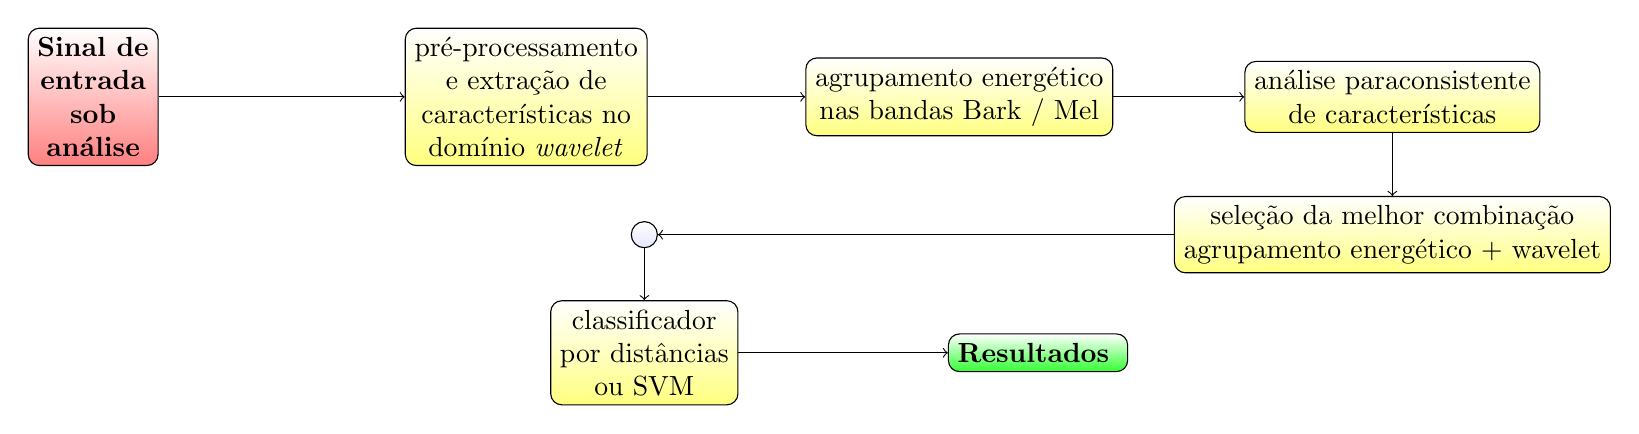
\begin{tikzpicture} 
			\node (z1)[shape=rectangle, rounded corners, draw, align=center, top color=white, bottom color=red!50] 
			at (0,2){
				\textbf{Sinal de} \\ \textbf{entrada} \\ \textbf{sob} \\ \textbf{análise}
			}; 
				
			\node (z2)[shape=rectangle, rounded corners, draw, align=center, top color=white, bottom color=yellow!50] 
			at (5.5,2){
				pré-processamento \\ e extração de \\ características no \\ domínio \textit{wavelet}
			}; 	
			
			\node (z3)[shape=rectangle, rounded corners, draw, align=center, top color=white, bottom color=yellow!50] 
			at (11,2){
				agrupamento energético \\ nas bandas Bark / Mel
			}; 	
			
			\node (z4)[shape=rectangle, rounded corners, draw, align=center, top color=white, bottom color=yellow!50] 
			at (16.5,2){
				análise paraconsistente \\ de características
			}; 
			
			\node (z5)[shape=rectangle, rounded corners, draw, align=center, top color=white, bottom color=yellow!50] 
			at (16.5,0.25){
				seleção da melhor combinação \\ agrupamento energético + wavelet
			}; 
					
			\node (z6)[shape=circle, draw, align=center, top color=white, bottom color=blue!10] 
			at (7,0.25) {};
			
			\node (z7)[shape=rectangle, rounded corners, draw, align=center, top color=white, bottom color=yellow!50] 
			at (7,-1.25) {
				classificador \\ por distâncias \\ ou SVM
			};
			
			\node (z8)[shape=rectangle, rounded corners, draw, align=center, top color=white, bottom color=green!80] 
			at (12,-1.25) {
				\textbf{Resultados}
			};
			
			\path[->] (z1) edge (z2);
			\path[->] (z2) edge (z3);
			\path[->] (z3) edge (z4);
			\path[->] (z4) edge (z5);
			\path[->] (z5) edge (z6);
			\path[->] (z6) edge (z7);	
			\path[->] (z7) edge (z8);
		\end{tikzpicture}
	}
	\label{fig_arq}
	\\Fonte: Elaborado pelo autor, 2021.
\end{figure}
			}
			\legend{Fonte: Elaborado pelo autor, 2024.}
			\label{fig:estruturaDaEstrategiaProposta}
		\end{figure}
	
		\subsection{Coleta dos dados}
			\par A coleta dos dados será realizada com software próprio desenvolvido para esse fim e com equipamentos de captação de voz e eletroencefalograma (EEG), montados a partir de componentes eletrônicos pré-fabricados, como placas de circuito integrado, eletrodos e microfones.
	
		\subsection{Extração de Características}
		
			\par A extração de características será realizada de duas maneiras:
			
			\begin{enumerate}
				\item \textbf{Método Manual (Handcrafting):} Características serão extraídas e formatadas por meio de métodos manuais de avaliação usando DTWT e a engenharia paraconsistente de características.
				\item \textbf{Método Automatizado:} Características serão extraídas utilizando redes neurais profundas, mais especificamente autoencoders.
			\end{enumerate}
			
			\par Dessa forma, além de avaliar quais características contribuem mais para a acurácia na autenticação biométrica, será possível comparar a abordagem manual com a automatizada.
			
			\par A confecção dos vetores de características, tanto no método manual quanto no automatizado, utilizará transformadas \textit{wavelet}, cálculos de energia nas frequências alvo e avaliação dos vetores por meio da engenharia paraconsistente de características.
			
		\subsection{Métricas}
		
			\par Afim de garantir a comparação do estudo com outros serão adotadas as seguintes métricas:
			
			\begin{itemize}
				\item acurácia
				\item pontuação F1
				\item precisão
				\item recall
				\item Erro Médio Quadrático
				\item área sob a Curva ROC
				\item sensitividade
				\item especificidade
			\end{itemize}
			
		\subsection{Desenvolvimento e Validação de Algoritmos}
		
			\par Quanto aos algoritmos de classificação, serão utilizadas redes neurais de pulso (SNN) em uma arquitetura de rede neural residual. Serão construídos modelos com o objetivo de minimizar o gasto de energia, memória e processamento, adequando-se a dispositivos com baixo poder computacional para garantir portabilidade e eficiência energética. Esses classificadores serão testados por meio de experimentos controlados (como exposto no início dessa seção) e comparados posteriormente com trabalhos do estado-da-arte.
			
	\section{Cronograma}
		\label{sec:cronograma}
	
		\begin{table}[h!]
			\centering
			\caption{Datas dos trabalhos a serem realizados}
			\begin{tabular}{|p{10cm}|c|c|}
				\hline
				\textbf{Etapa} & \textbf{Início} & \textbf{Fim} \\
				\hline
				Programação do sistema de coleta de dados & 01/09/2024 & 01/12/2024 \\
				\hline
				Criação da base de dados & 01/01/2025 & 01/12/2025 \\
				\hline
				Extração e seleção de características & 01/02/2025 & 01/12/2025 \\
				\hline
				Desenvolvimento de classificadores & 01/12/2025 & 01/12/2026 \\
				\hline
				Validação experimental e comparação & 01/03/2026 & 01/02/2027 \\
				\hline
				Divulgação e publicação dos resultados & 01/02/2027 & 01/04/2027 \\
				\hline
				Redação da dissertação e preparação para defesa & 01/09/2024 & 01/03/2027 \\
				\hline
			\end{tabular}
			\label{tab:cronograma}
		\end{table}
		
		\begin{table}[h!]
			\centering
			\caption{Gráfico de Gantt dos trabalhos a serem realizados}
			\begin{ganttchart}[
				hgrid, % Adiciona linhas horizontais de grade para melhorar a legibilidade do gráfico
				vgrid, % Adiciona linhas verticais de grade
				x unit=.455cm, % Define a largura de cada unidade de tempo (neste caso, um mês) em centímetros
				y unit chart=0.8cm, % Define a altura de cada linha de tarefa no gráfico em centímetros
				bar/.append style={fill=green, draw=green}, % Estilo padrão para as barras: cor de preenchimento verde e borda verde
				bar label font=\scriptsize\bfseries, % Define o estilo da fonte para os rótulos das barras (pequeno e em negrito)
				bar label node/.append style={text=black, anchor=west, xshift=0.2cm}, % Alinha o texto da barra ao início da barra com um pequeno deslocamento horizontal
				group label node/.append style={anchor=east, font=\small}, % Define o estilo dos rótulos de grupo com ânfora à esquerda e fonte pequena
				time slot format=isodate, % Define o formato de data para os slots de tempo (ISO: ano-mês-dia)
				milestone/.append style={fill=green}, % Estilo para marcos: preenchimento verde
				title/.append style={fill=blue, draw=black}, % Estilo do título: preenchimento azul e borda preta
				title label font=\bfseries\footnotesize, % Define o estilo da fonte para os rótulos do título (pequeno e em negrito)
				title label anchor/.style={below=0ex}, % Ajusta a âncora do rótulo do título para baixo
				title/.style={fill=blue!30, draw=none}, % Estilo do título: preenchimento azul claro e sem borda
				title label font=\scriptsize\bfseries, % Define o estilo da fonte para os rótulos do título (pequeno e em negrito)
				milestone label font=\small\bfseries, % Define o estilo da fonte para os rótulos de marcos (pequeno e em negrito)
				bar height=0.5, % Define a altura das barras
				time slot unit=month, % Define a unidade de tempo como mês
				y unit title=0.9cm % Define a altura da linha do título em centímetros
				]{2024-08-10}{2027-05-01} % Define o intervalo de datas para o gráfico Gantt
				
				\gantttitlecalendar{year, month=number} \\ % Adiciona um título de calendário ao gráfico, mostrando ano e número do mês
				
				% Define as barras de tarefas com seus rótulos e datas de início e fim
				\ganttbar[
				bar label node/.append style={xshift=6pt} % Ajusta o texto da barra para começar no início da barra
				]{Programação do sistema de coleta de dados}{2024-09-01}{2024-12-01} \\
				\ganttbar[
				bar label node/.append style={xshift=57pt} % Ajusta o texto da barra para começar no início da barra
				]{Criação da base de dados}{2025-01-01}{2025-12-01} \\
				\ganttbar[
				bar label node/.append style={xshift=70pt} % Ajusta o texto da barra para começar no início da barra
				]{Extração e seleção de características}{2025-02-01}{2025-12-01} \\
				\ganttbar[
				bar label node/.append style={xshift=200pt} % Ajusta o texto da barra para começar no início da barra
				]{Desenvolvimento de classificadores}{2025-12-01}{2026-12-01} \\
				\ganttbar[
				bar label node/.append style={xshift=240pt} % Ajusta o texto da barra para começar no início da barra
				]{Validação experimental e comparação}{2026-03-01}{2027-02-01} \\
				\ganttbar[
				bar label node/.append style={xshift=230pt} % Ajusta o texto da barra para começar no início da barra
				]{Divulgação e publicação dos resultados}{2027-02-01}{2027-04-01} \\
				\ganttbar[
				bar/.append style={fill=orange}, % Altera a cor da barra para laranja
				bar label node/.append style={xshift=4pt} % Ajusta o texto da barra para começar no início da barra
				]{Redação da dissertação e preparação para defesa}{2024-09-01}{2027-03-01}
			\end{ganttchart}
			\label{tab:cronogramaGantt}
		\end{table}

\section{Resultados Esperados}

	\par Espera-se desenvolver algoritmos de extração de características e classificação para voz e eletroencefalograma (EEG) que aprimorem a acurácia na identificação de indivíduos. Além disso, serão avaliadas se as alegações sobre o consumo energético e a eficácia das redes neurais de pulso (SNN) na classificação de informações temporais são confirmadas para o problema estudado. Será constituída uma base de dados contendo sinais de voz, EEG e sinais mistos que deve ser disponibilizada ao público. Por fim, pretende-se comparar o desempenho das técnicas de extração de características manuais com as automatizadas.


%\section{Procedimentos}
%\subsection{Tratamento do sinal}
%\subsection{Procedimento 01}